\documentclass[final,hyperref={pdfpagelabels=false}]{beamer}
\usepackage{grffile}
\mode<presentation>{\usetheme{_bauer}}
\usepackage[english]{babel}
\usepackage[latin1]{inputenc}
\usepackage{amsmath, amsthm, amssymb, latexsym}

%\usepackage{times}\usefonttheme{professionalfonts}  % obsolete
%\usefonttheme[onlymath]{serif}
%\boldmath % macht ALLE Gleichungen automatisch fett
\usepackage[orientation=portrait,size=a0,scale=1.4,debug]{beamerposter}
% change list indention level
% \setdefaultleftmargin{3em}{}{}{}{}{}



% Eigene Befehle und Einstellungen -------------------------
\newcommand{\bfBlue}[1]{\textcolor{koaladarkestblue}{\textbf{#1}}}
% Numbers with circles around it for headers
\usepackage{tikz}
\newcommand*\circled[1]{\tikz[baseline=(char.base)]{
\node[shape=circle,draw,inner sep=2pt] (char) {#1};}}
% Make figures get numbers (Figure 1, ...)
\setbeamertemplate{caption}[numbered]
% Change style of figure caption label
\usepackage[font={footnotesize,it,color=black}]{caption}
\captionsetup[figure]{labelfont={color=black}}
\captionsetup[figure]{labelfont=bf}
% Highlight text parts with a color block with rounded corners
\usepackage{tcolorbox}
\newtcbox{\mybox}{nobeforeafter,colframe=chocolate4,colback=verylightgray,boxrule=2pt,arc=4pt,
  boxsep=0pt,left=6pt,right=6pt,top=6pt,bottom=6pt,tcbox raise base}
% Eigene Befehle Ende --------------------------------------



%\usepackage{snapshot} % will write a .dep file with all dependencies, allows for easy bundling

\usepackage{array,booktabs,tabularx}
\newcolumntype{Z}{>{\centering\arraybackslash}X} % centered tabularx columns
\newcommand{\pphantom}{\textcolor{ta3aluminium}} % phantom introduces a vertical space in p formatted table columns??!!
  
  \listfiles

%%%%%%%%%%%%%%%%%%%%%%%%%%%%%%%%%%%%%%%%%%%%%%%%%%%%%%%%%%%%%%%%%%%%%%%%%%%%%%%%%%%%%%
\graphicspath{{figures/}}

\title{\huge{KOALA: Estimating coalition probabilities}\\[0.5ex]\LARGE{in multi-party electoral systems}}
\author{Alexander Bauer$^{1}$, Andreas Bender$^{1}$, Andr\'e Klima$^{1}$, Helmut K\"{u}chenhoff$^{1}$}
\institute[LMU Munich]{\textit{$^{1}$ Statistical Consulting Unit StaBLab, Department of Statistics, LMU Munich,
Germany} \\[2ex] \texttt{Alexander.Bauer@stat.uni-muenchen.de}}
\date[July 18th, 2018]{July 18th, 2018}

%%%%%%%%%%%%%%%%%%%%%%%%%%%%%%%%%%%%%%%%%%%%%%%%%%%%%%%%%%%%%%%%%%%%%%%%%%%%%%%%%%%%%%
  \newlength{\columnheight}
\setlength{\columnheight}{105cm}


%%%%%%%%%%%%%%%%%%%%%%%%%%%%%%%%%%%%%%%%%%%%%%%%%%%%%%%%%%%%%%%%%%%%%%%%%%%%%%%%%%%%%%

% Begin page ----------------------------------------------
\begin{document}
\begin{frame}
\begin{columns}
\begin{column}{1\textwidth} % 1 Seite, die die ganze Seite einnimmt


% Application ---------------------------------------------
\begin{beamercolorbox}[center,wd=\textwidth]{postercolumn}
\begin{minipage}[T]{.95\textwidth}  % tweaks the width, makes a new \textwidth
\begin{block}{\footnotesize Data and Research Question}
  \begin{columns}[t]
  \begin{column}{.6\textwidth}
  \vspace{-3ex}
  \begin{center}
  \bfBlue{Setting}
  \end{center}
  We analyze artificial earthquake data derived from large-scale computer simulations based on a 1994 earthquake in Northridge (USA). In each of 135 simulations, the (isotropic) \bfBlue{absolute ground velocity} [m/s] was measured at 6146 virtual seismograms with a temporal resolution of 2Hz.
  \\[2ex]
  This project marks the first time that physics-based simulations of earthquakes are combined with modern statistical methods. Apart from gaining new insights in the geophysical processes regression models could in future be used to predict expected ground movements in earthquake regions.
  \\[4ex]
  \begin{tabularx}{\textwidth}{ZZ}
  \raggedright \bfBlue{Main research question}
  \\[0.35ex] % align the following text block horizontally with the itemize in the other column
  How do the physical conditions at an earthquake fault affect the surficial ground velocity measured over time?
  &
  \raggedright \bfBlue{Challenges}
  \begin{itemize}
    \item Very high-dimensional data
    \item Spatio-temporal functional data
  \end{itemize}
  
  \end{tabularx}
  \vspace{2ex}
  \begin{figure}[!ht]\centering
  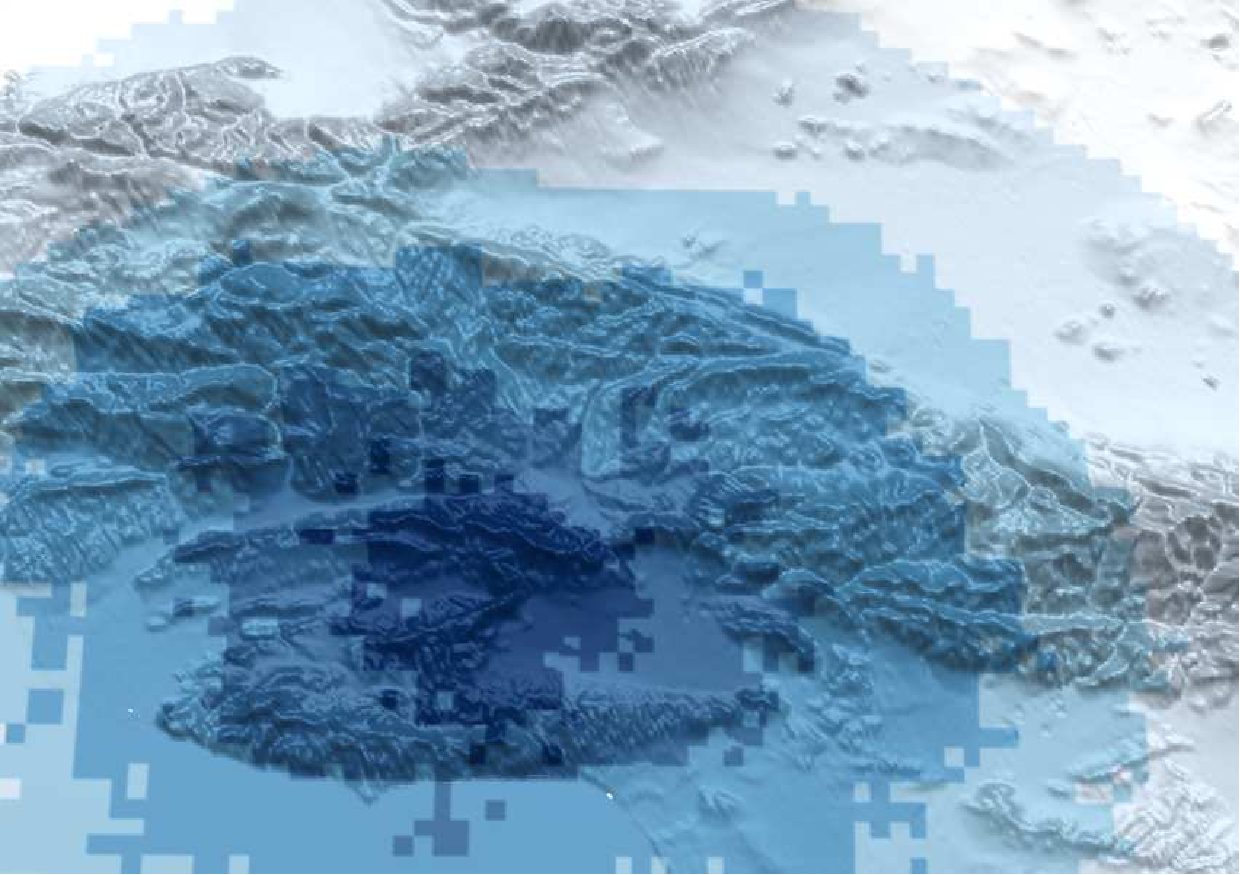
\includegraphics[width=0.2\linewidth]{figures/bauer_73_gm_3D_ausschnitt.pdf}
  \hspace{5ex}
  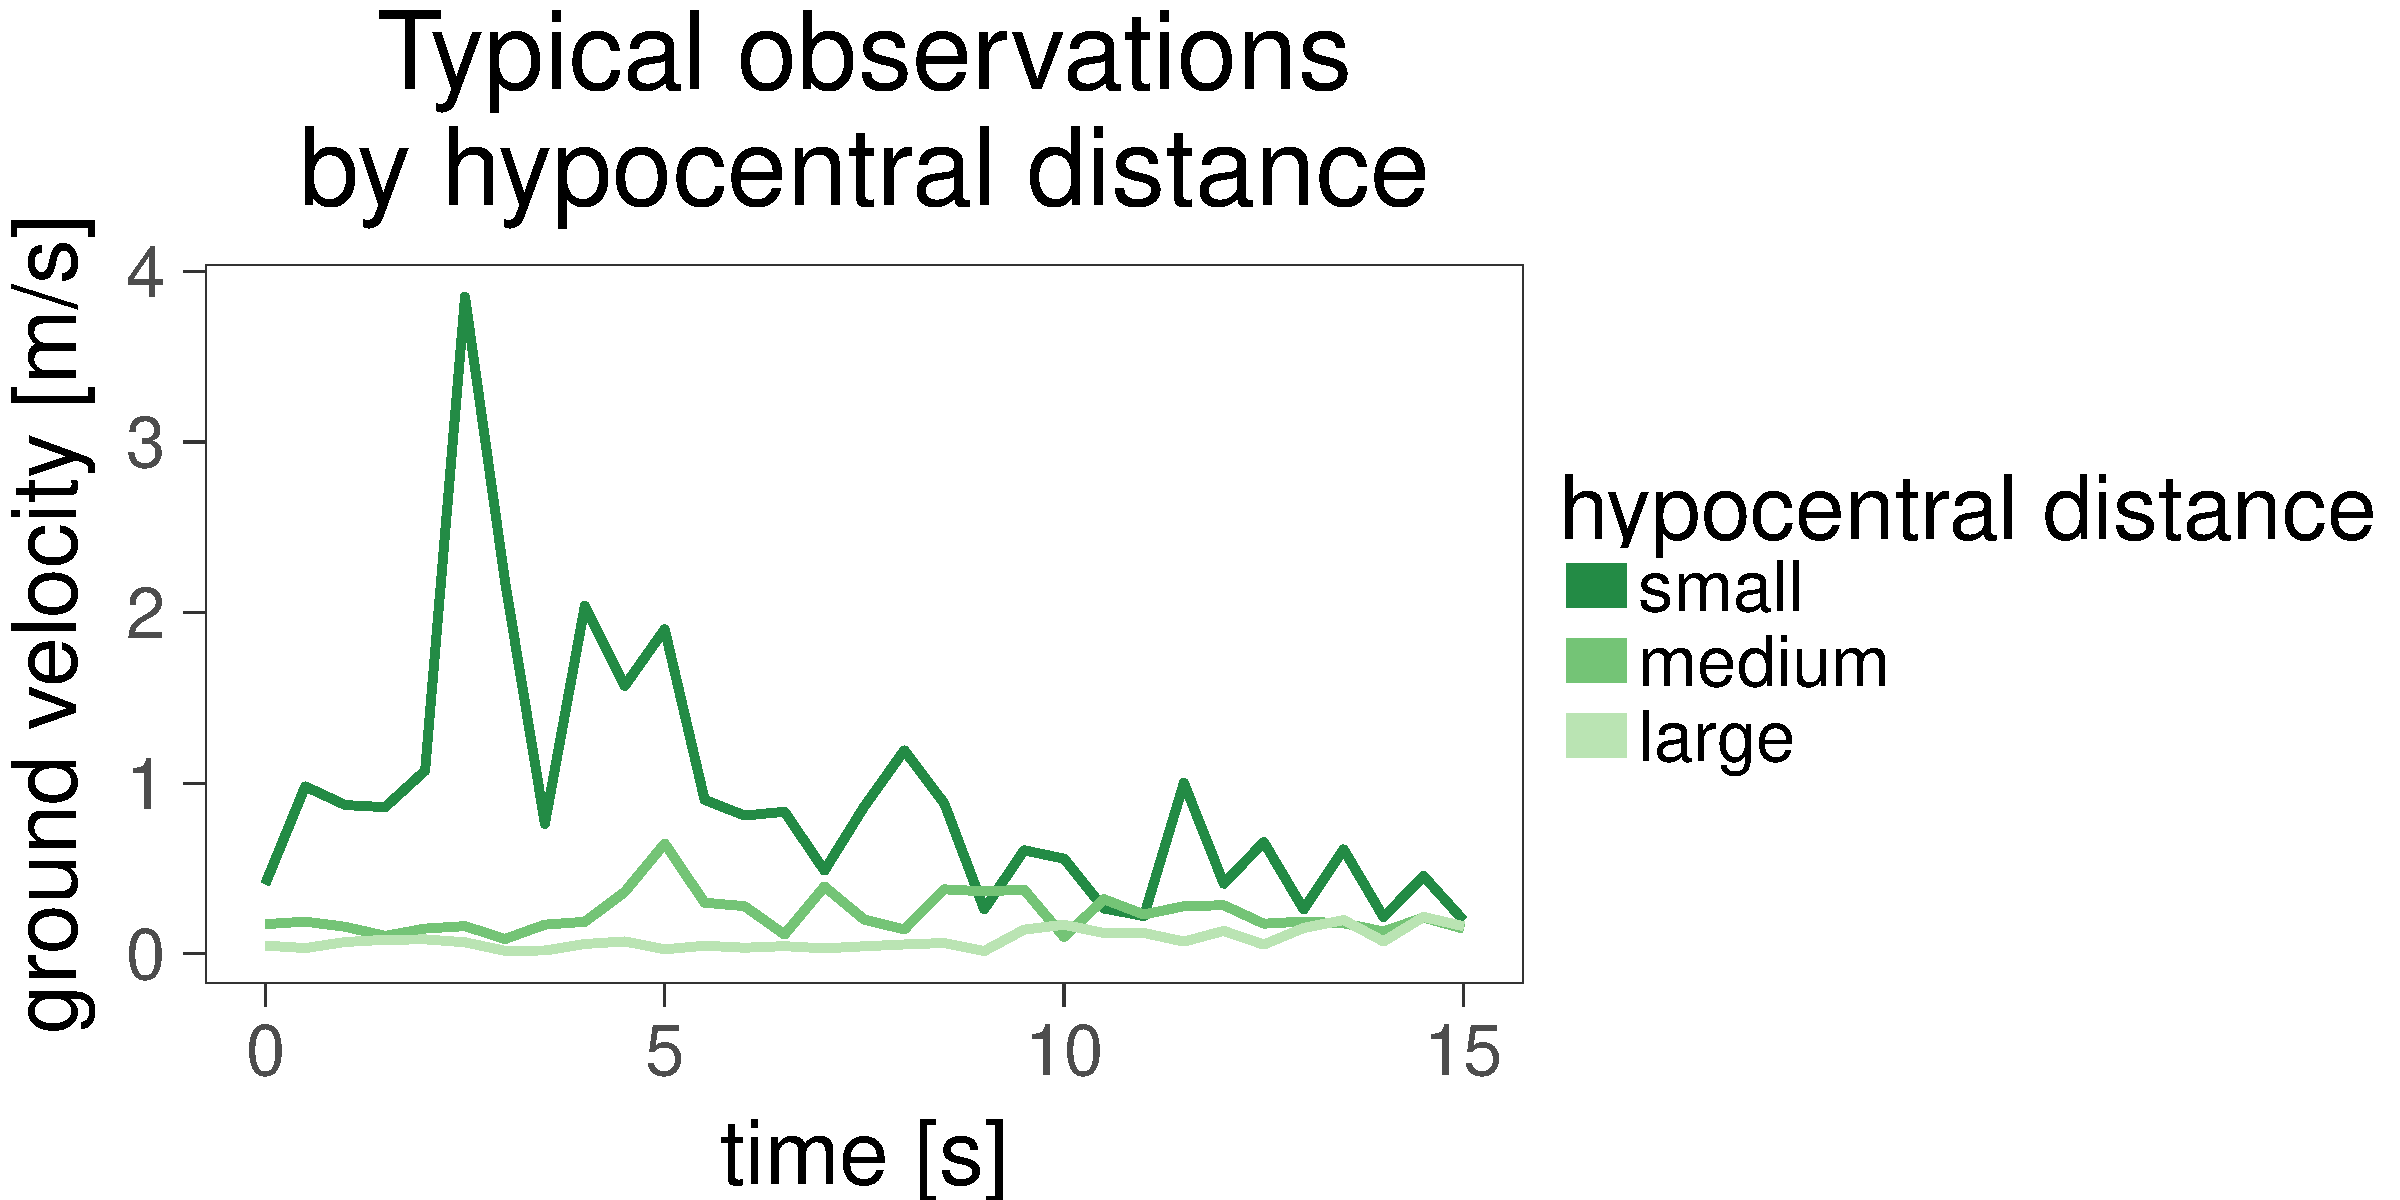
\includegraphics[width=0.27\linewidth]{figures/motivation2.pdf}
  \caption{\footnotesize Left: Categorized mean absolute ground velocity in one simulation over the area under study, darker colours correspond to increased velocity. Right: Typical observations of absolute ground velocity over time. The initial peak of the ground velocity is delayed and smaller as hypocentral distance increases.}
  \end{figure}
  \end{column}
  
  \hspace{-1.5ex}
  \textcolor{LMUlightgray}{\vrule{}}
  \hspace{1.5ex}
  
  \begin{column}{.35\textwidth}
  \vspace{-3ex}
  \begin{center}
  \bfBlue{Simulation setup}
  \end{center}
   The artificial earthquake data were generated using the open-source software SeisSol (\texttt{www.seissol.org}). In each simulation:
  \begin{enumerate}
    \item Five \mybox{simulation parameters} were pre-set, and
    \item absolute ground velocities were simulated solving elastic wave equations coupled to frictional failure at the earthquake fault.
  \end{enumerate}
  \vspace{2ex}
  \begin{center}
  \bfBlue{Influence parameters}
  \end{center}
  The influence parameters are all \bfBlue{constant over time}.
  \hspace{-2pt}
  \begin{tcolorbox}[colframe=chocolate4,colback=verylightgray,boxrule=2pt,arc=4pt,
  left=-5pt]
  % {nobeforeafter,colframe=niceblue,colback=lightgray,boxrule=2pt,arc=4pt,
  % boxsep=0pt,left=6pt,right=6pt,top=6pt,bottom=6pt,tcbox raise base}
  \begin{itemize} \footnotesize
    \item soil material (\{$rock$, $sediment$\})
    \item linear slip weakening distance [m]
    \item static coefficient of friction
    \item dynamic coefficient of friction
    \item direction of tectonic background stress [$^\circ$]
  \end{itemize}
  \end{tcolorbox}
  \vspace{-10px}
  \begin{itemize} \footnotesize
    \item hypocentral distance of seismometer [m]
    \item elevation of seismometer [m]
    \item landform at seismometer$^\ast$ (\{$ridge$, $plain$, $valley$, \ldots\})
    \item moment magnitude [Nm]
  \end{itemize}
  \vspace{1ex}
  {\footnotesize $^\ast$Categorization into landforms was performed using the Topographic Position Index (TPI) of Weiss (2001)}
  \end{column}
  \end{columns}
  \vskip-1ex
\end{block}
\end{minipage}
\end{beamercolorbox}



% Begin main part -----------------------------------
\vspace{2ex}
\begin{columns}[T]

% empty space on left
\begin{column}{.016\textwidth}
\end{column}

\begin{column}{.484\textwidth}
\begin{beamercolorbox}[center,wd=\textwidth]{postercolumn}
\begin{minipage}[T]{.95\textwidth}  % tweaks the width, makes a new \textwidth
% \parbox[t][\columnheight]{\textwidth}{ % must be some better way to set the the height, width and textwidth simultaneously
% Since all columns are the same length, it is all nice and tidy.  You have to get the height empirically

% Modeling process ---------------------------------------
\begin{block}{\footnotesize \circled{1} Modeling process}
\begin{minipage}[T]{.95\textwidth}  % tweaks the width, makes a new \textwidth
\vspace{1ex}
We use a \bfBlue{Generalized Functional Additive Model} (GFAM) (see Scheipl et al., 2016) which is an extension of the GAM model class.
\\
In our case, only the response is functional and we use a Gamma model with log-link.
\\
$$
y_i(t_l) \sim F(\mu_{il}, \boldsymbol{\nu}) \text{\ \ with\ \ } g(\mu_{il}) = \beta_0(t) + \sum\limits_{r=1}^R f_r(\boldsymbol{\mathcal{X}}_{ri}, t_l), \ \ \ i = 1,\ldots,n
$$
\begin{itemize}
  \item $y_i(t_l)$: Value of functional response observed at time point $t_l$
  \item $F(\mu_{il}, \boldsymbol{\nu})$: Conditional distribution of $y_i(t_l)$ with conditional expectation $\mu_{il}$ and shape parameters $\boldsymbol{\nu}$
  \item $g(\cdot)$: Link function
  \item $\beta_0(t)$: Functional intercept
  \item $f_r(\boldsymbol{\mathcal{X}}_{ri}, t_l)$: One of $R$ additive effects with associated covariates $\boldsymbol{\mathcal{X}}_{ri}$ and potentially varying over the functional time domain $t$
  \item $n$: number of functional observations
\end{itemize}
\vspace{2ex}

\noindent \textcolor[RGB]{220,220,220}{\rule{0.9\linewidth}{3pt}}
\vspace{2ex}

\noindent
We use a \bfBlue{highly performant estimation algorithm} from Wood et al. (2016) to make estimation of this complex model on such large data feasible. Major advances are:
\begin{itemize}
  \item a block-wise Cholesky decomposition
  \item a compressed representation of marginal spline bases
\end{itemize}
\vspace{1ex}
A prediction error based approach was used for tuning basis sizes, resulting smooth effects were estimated using (tensor product) P-splines.
\end{minipage}
\end{block}


% Covariate effects -------------------------------------
\begin{block}{\footnotesize \circled{2} Covariate effects}
The hypocentral distance and the dynamic frictional resistance have by far the strongest effects, with higher values leading to decreased ground velocities for both.
\\[5.0ex]
\begin{tabularx}{.95\textwidth}{ZZZ!{\color{LMUdarkgray}\vrule{}}Z}
% & Hypocentral distance & & Dynamic coefficient of friction \\
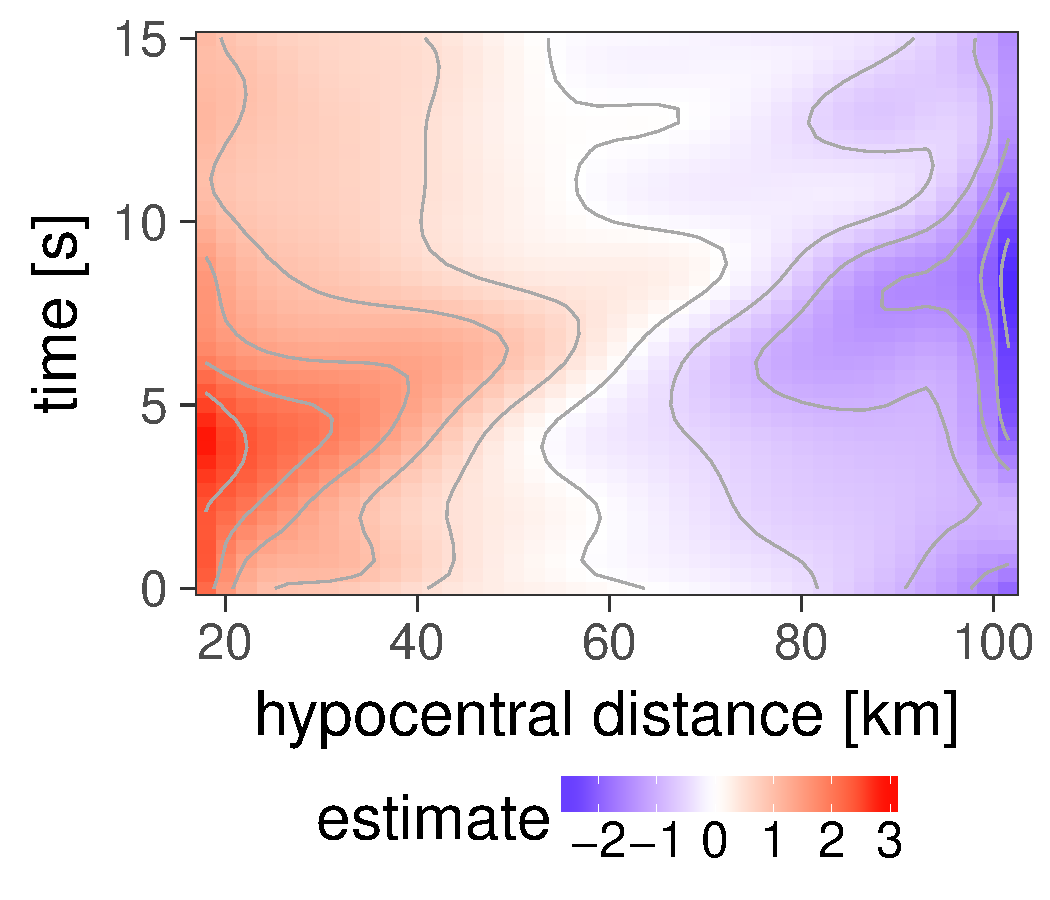
\includegraphics[width=.9\linewidth]{figures/Effekte_hypoDis1.pdf}
&
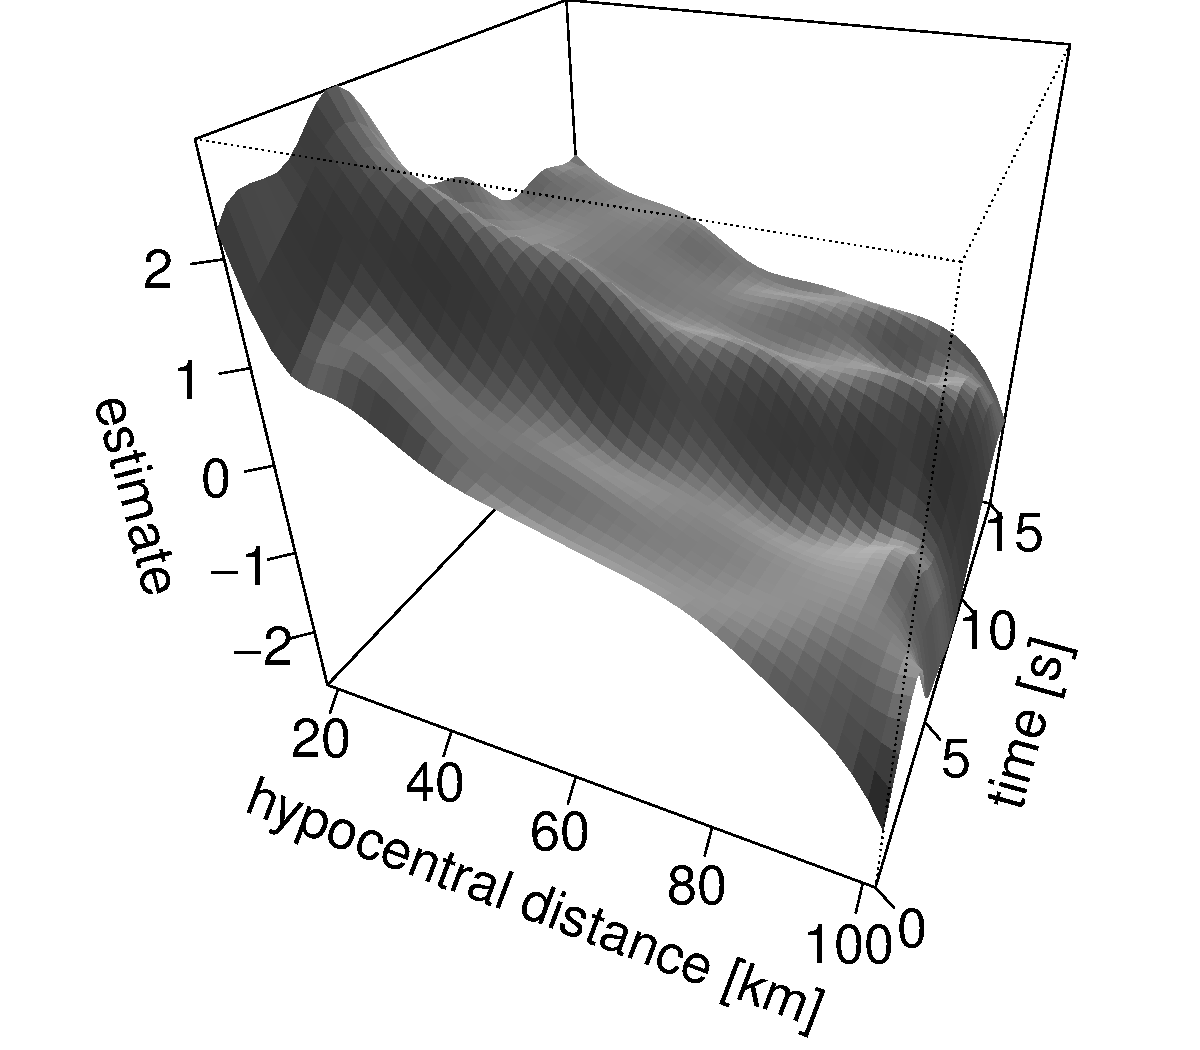
\includegraphics[width=.9\linewidth]{figures/Effekte_hypoDis2.pdf}
&
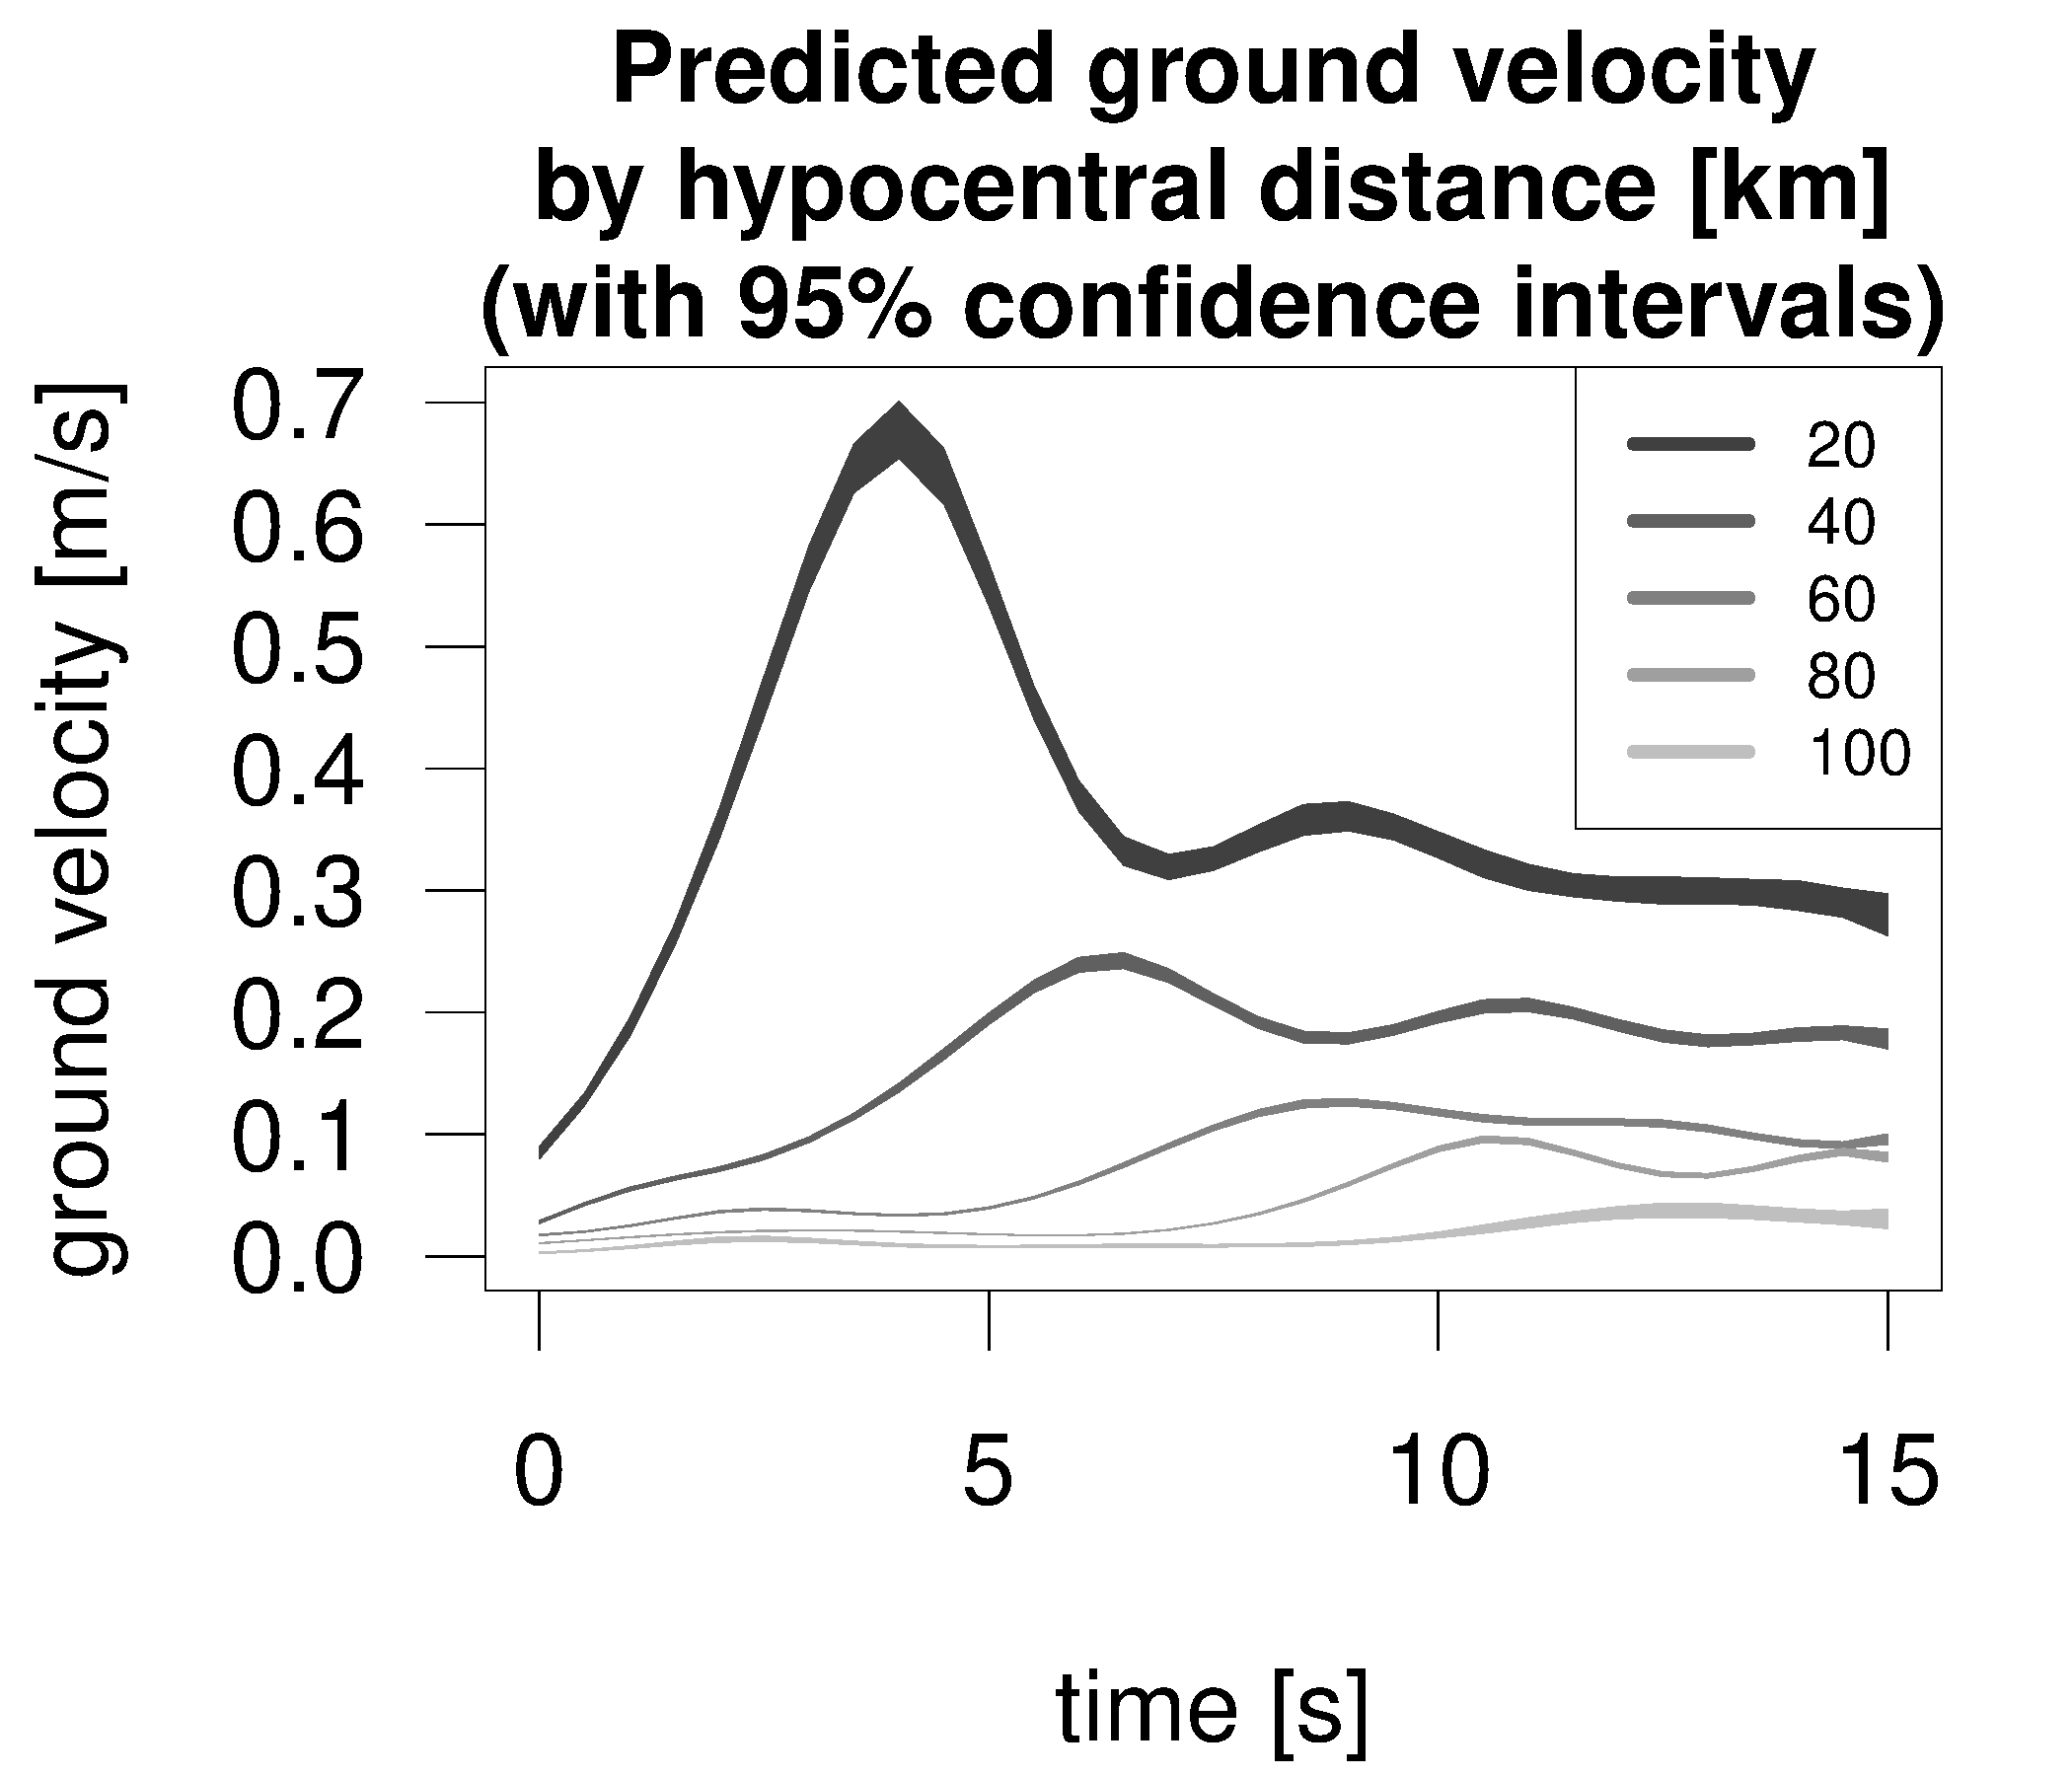
\includegraphics[width=.9\linewidth]{figures/Effekte_hypoDis3.pdf}
&
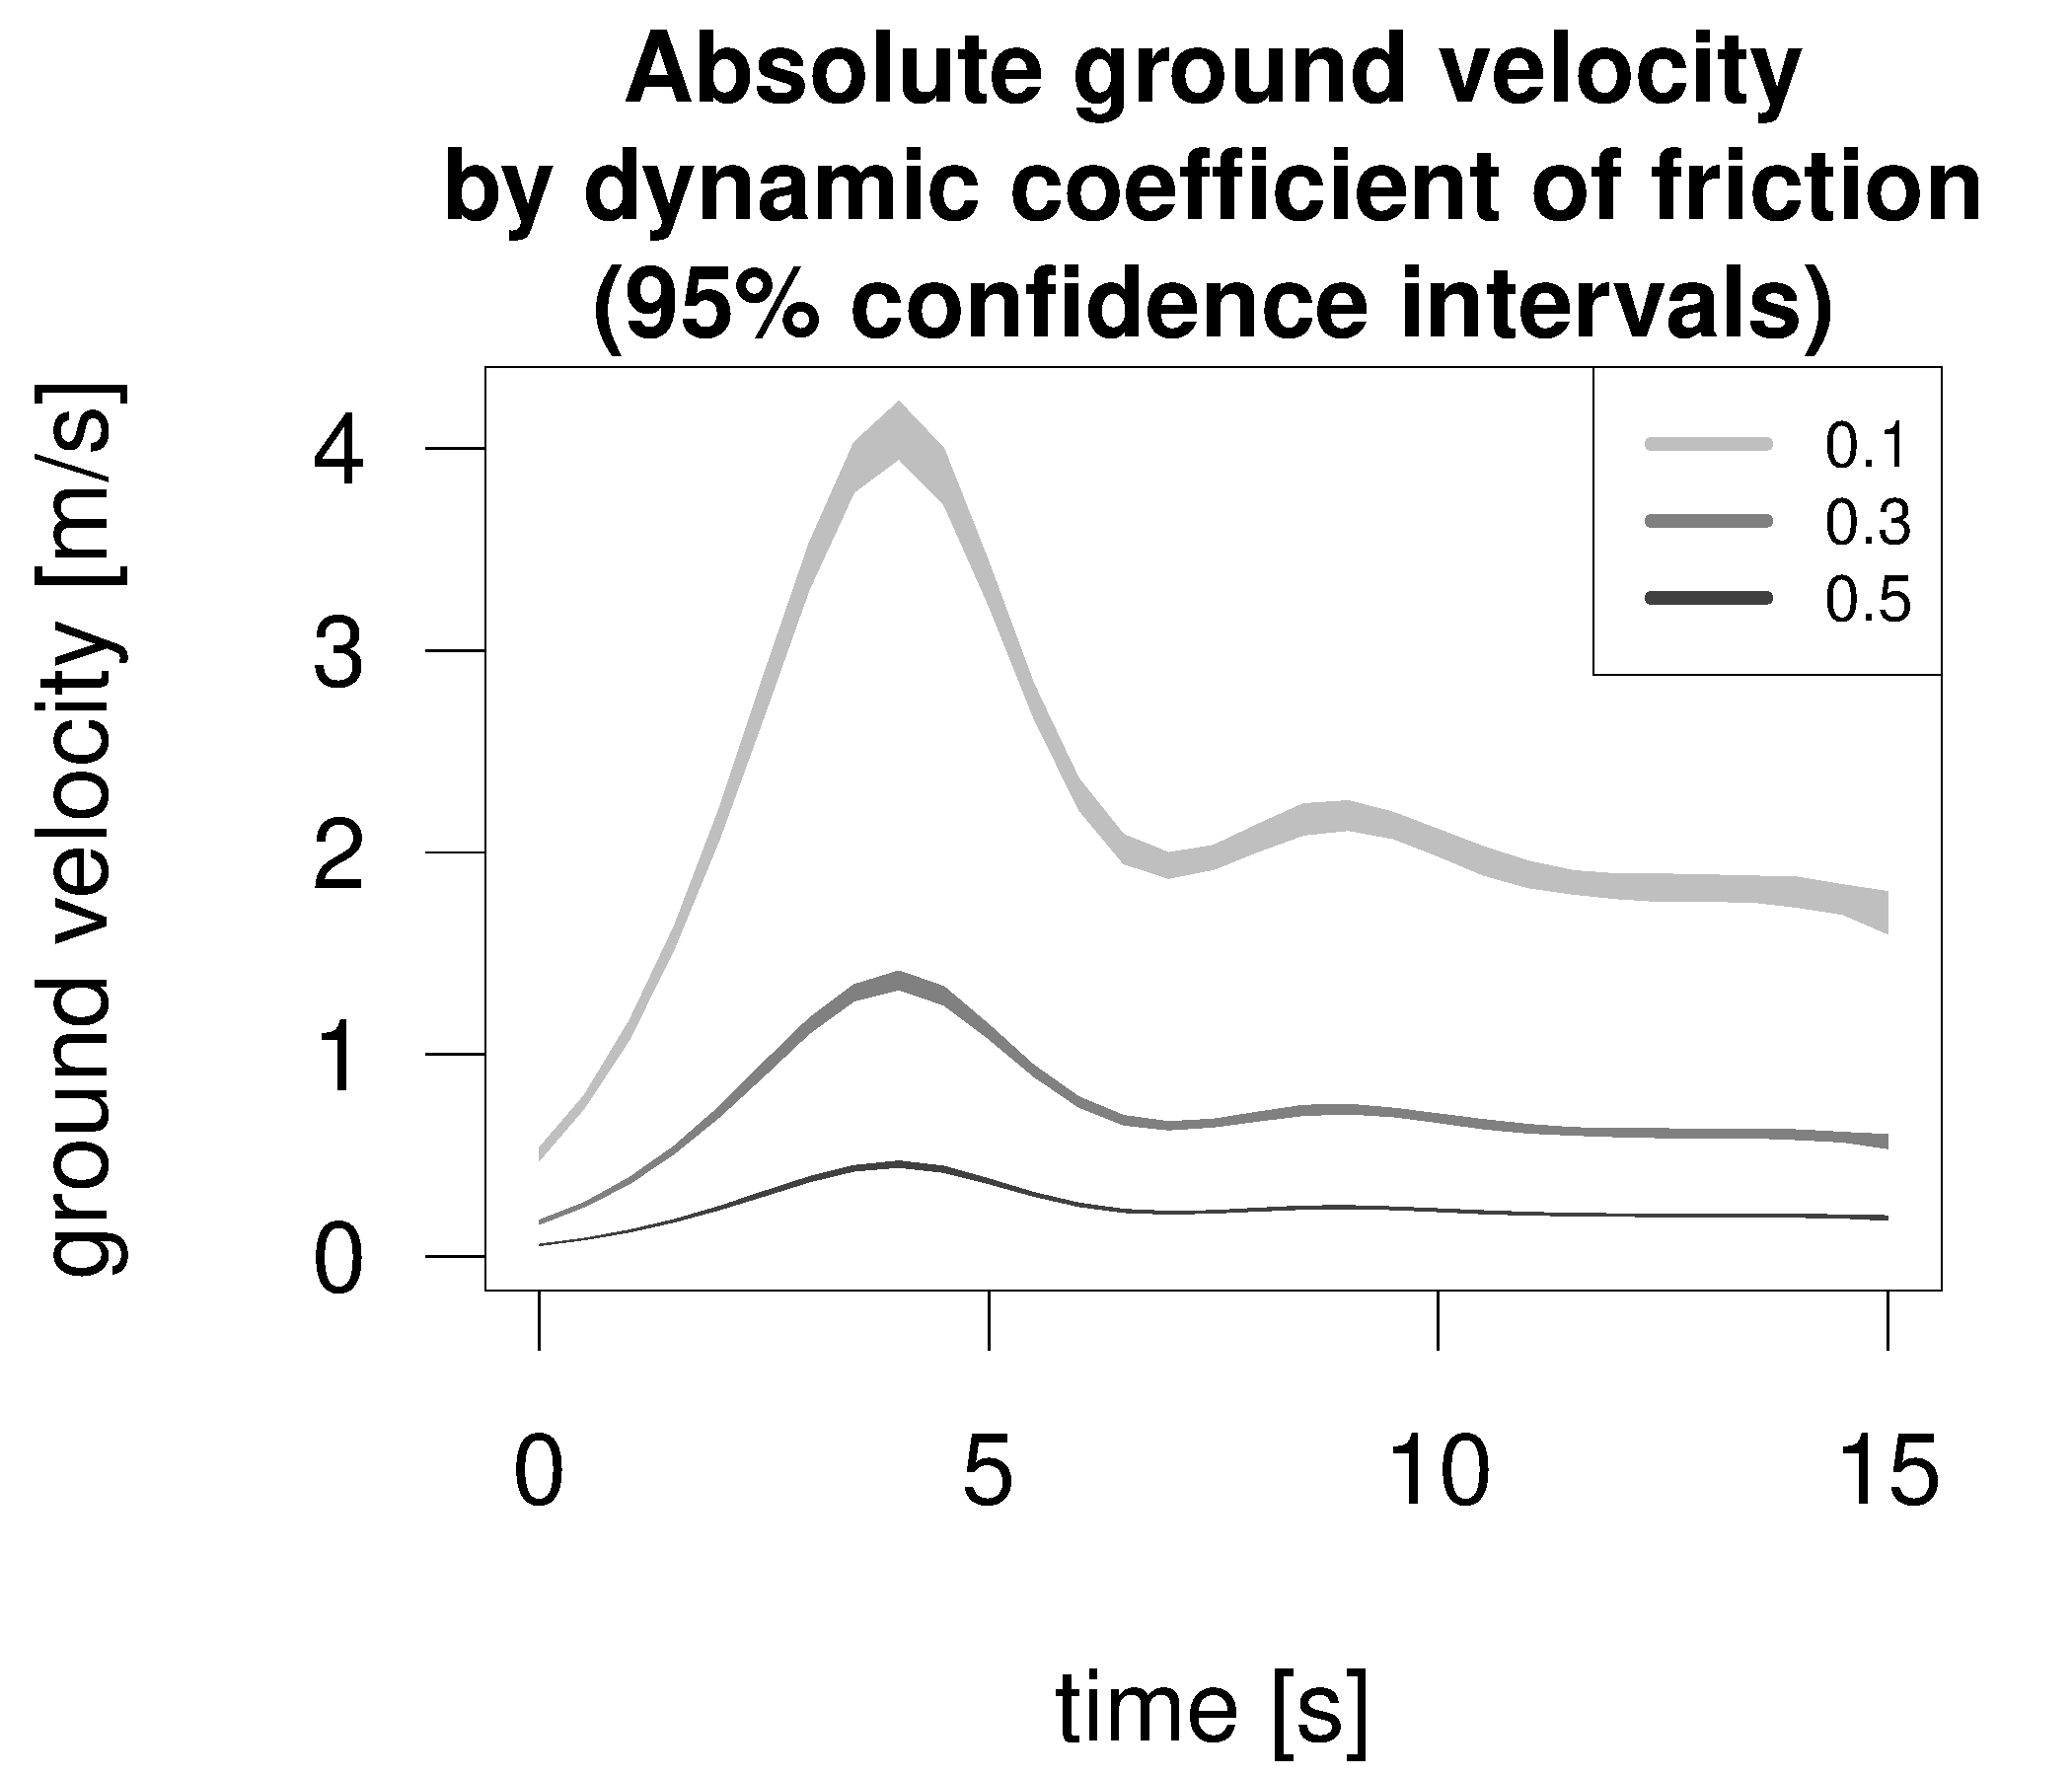
\includegraphics[width=.9\linewidth]{figures/Effekte_md1.pdf}
\\
\end{tabularx}
\vspace{-3.5ex}
\begin{center}
\begin{tabularx}{.97\textwidth}{Z}
\begin{figure}[!ht]\centering
\caption{\footnotesize Left: Nonlinear, time-varying effect of hypocentral distance as heatmap and 3D surface, and predictions based on varying hypocentral distances, while other covariates are held constant at realistic values.
Right: Predictions based on varying values of the dynamic coefficient of friction, which has a linear, time-constant effect of -5.48 \\
}
%Nonlinear, time-varying smooth effects of hypocentral distance (left) and the dynamic coefficient of friction (right) and model predictions based on varying values, while other covariates are held constant at realistic values.}
\end{figure}
\end{tabularx}
\end{center}
\vspace{-3ex}
\end{block}



% Begin second column of main part -----------------
\end{minipage}
\end{beamercolorbox}
\end{column}

\begin{column}{.484\textwidth}
\begin{beamercolorbox}[center,wd=\textwidth]{postercolumn}
\begin{minipage}[T]{.95\textwidth}  % tweaks the width, makes a new \textwidth


% Model evaluation & Conclusion -------------------
\begin{block}{\footnotesize \circled{3} Model evaluation}
\vspace{-3ex}
\begin{center}
\begin{tabularx}{0.975\linewidth}{Z}
  \begin{figure}[!ht]\centering
  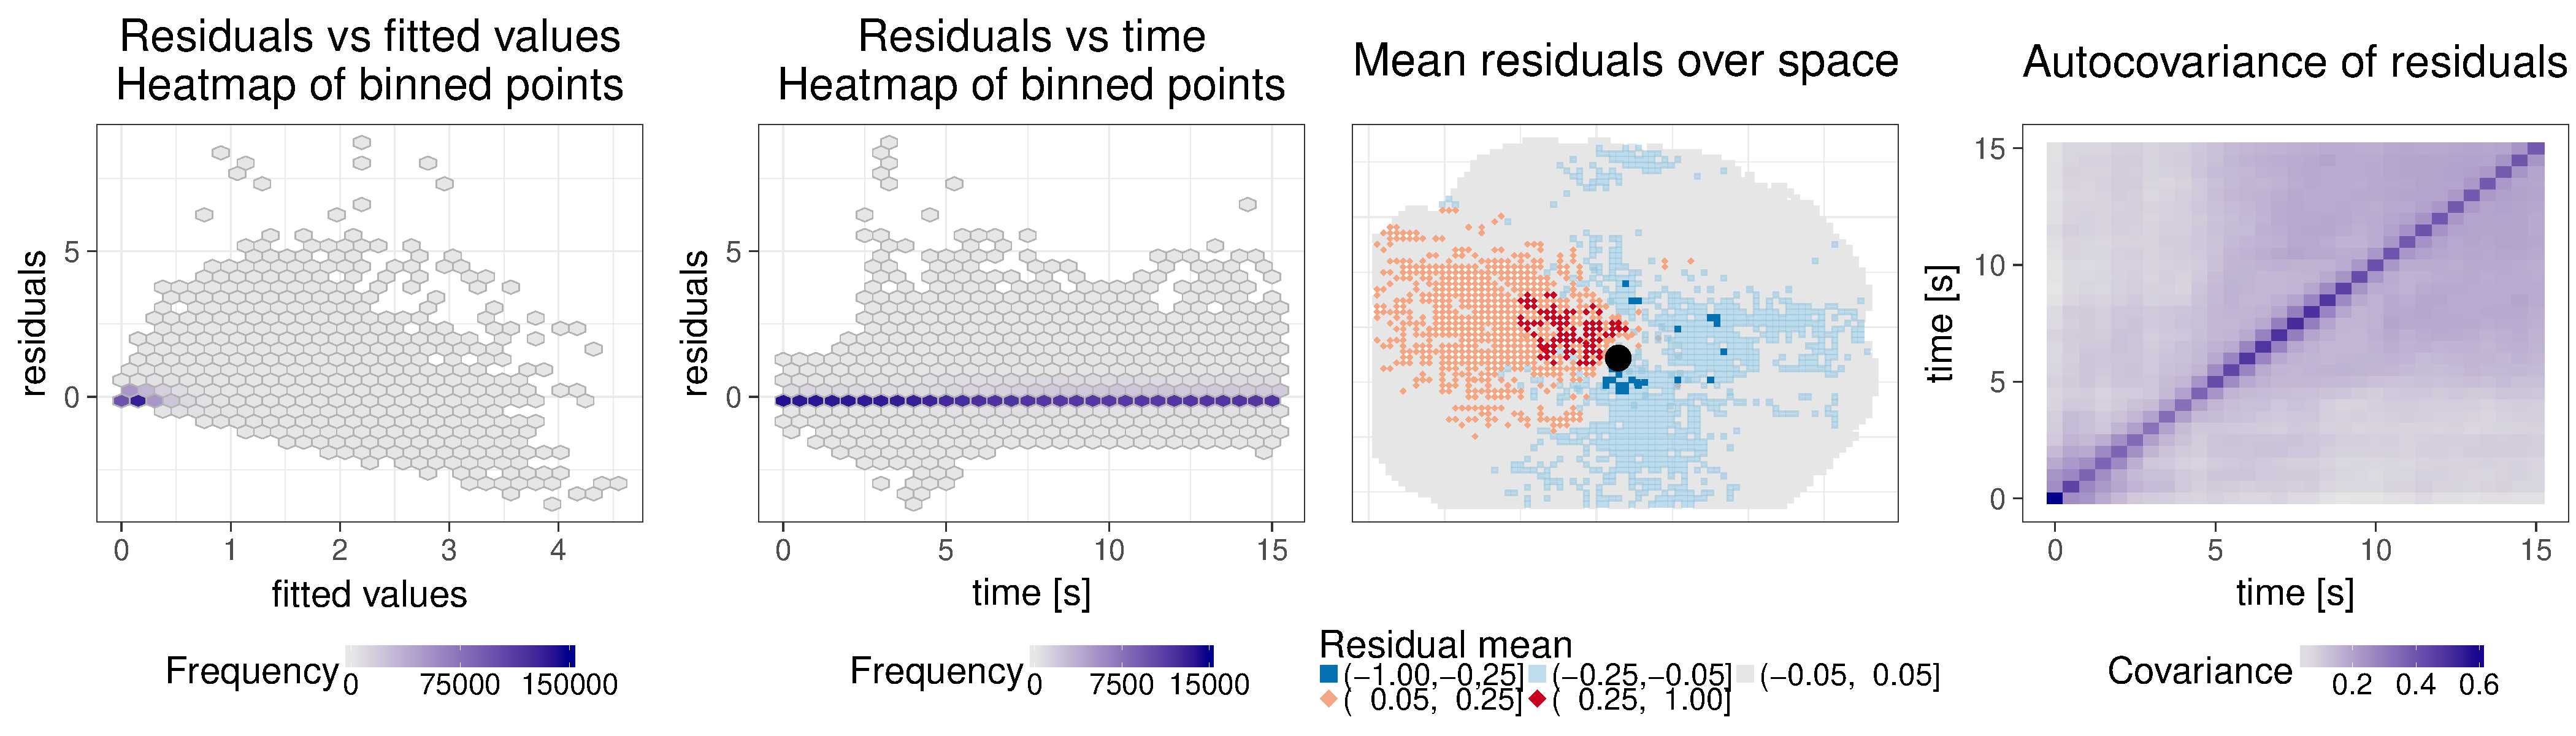
\includegraphics[width=0.8\linewidth]{figures/Residuen}
  \caption{\footnotesize From left to right: Residuals vs fitted values, residuals vs the time domain, residuals vs space, autocovariance of residuals over the functional domain. The black dot in the third plot marks the epicenter.}
  \end{figure}
\end{tabularx}
\end{center}

\vspace{-5ex}

\begin{center}
\begin{tabularx}{0.975\linewidth}{Z}
  \begin{figure}[!ht]\centering
  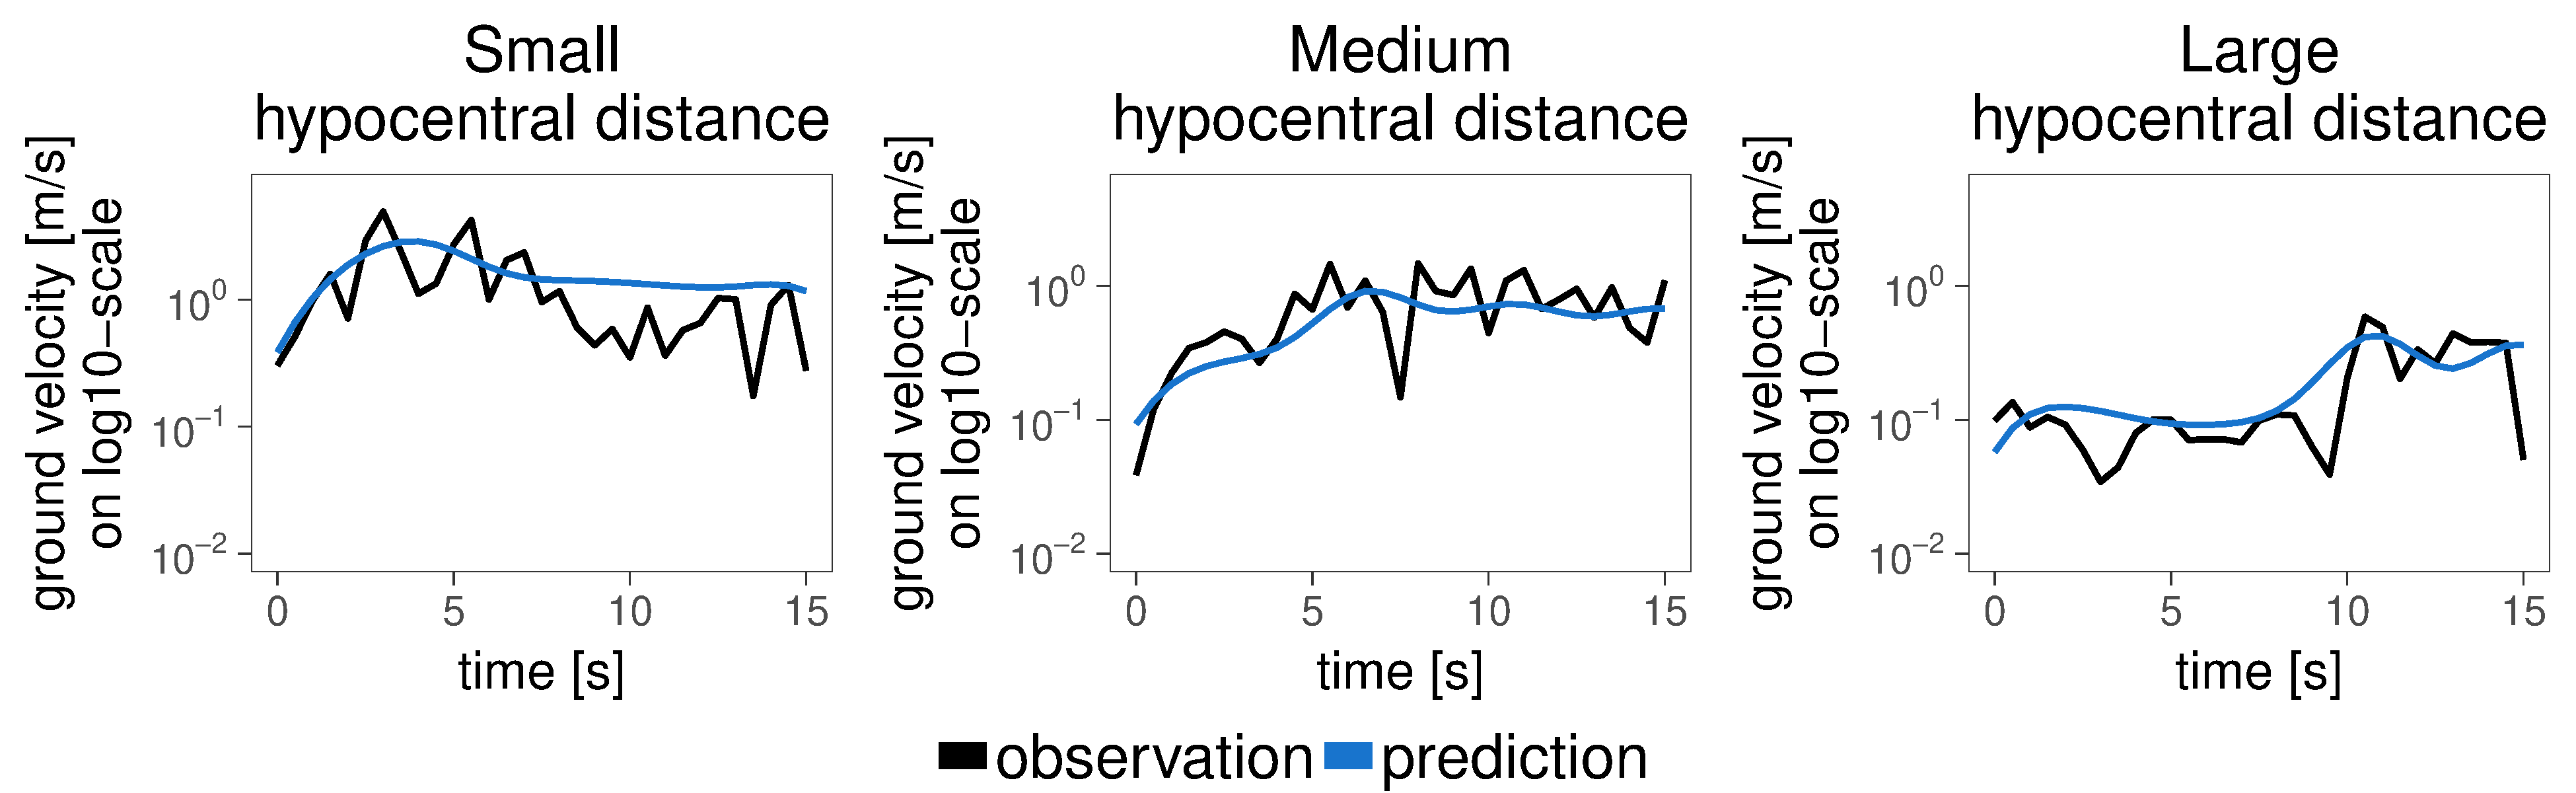
\includegraphics[width=0.6\linewidth]{figures/predictions}
  \caption{\footnotesize Comparison of model predictions and raw observations for typical observations with different hypocentral distances.}
  \end{figure}
\end{tabularx}
\end{center}

\vspace{-2ex}
\textcolor{koaladarkblue}{$\Rightarrow$} Spatial residual structure remaining \\[0.15cm]
\textcolor{koaladarkblue}{$\Rightarrow$} Predictions in general behave well (70.7\% explained null deviance)

% \vspace{3ex}
% \noindent \textcolor[RGB]{220,220,220}{\rule{0.9\linewidth}{3pt}}
% \vspace{2ex}
% \begin{center}
% \bfBlue{Results}
% \end{center}
\end{block}

\begin{block}{\footnotesize \circled{4} Conclusion \& Outlook}
\begin{minipage}[T]{.95\textwidth}  % tweaks the width, makes a new \textwidth
\vspace{1ex}
Functional additive regression models are a promising approach for modeling surficial ground velocity.
\\[2.4ex]
\bfBlue{Our model}
\begin{itemize}
  \item allows a better understanding of the observed seismological patterns
  \item adds value to the current seismological discussion of how important precise determination of specific physical parameters is
  \item offers predictions which could in future replace computer-intensive earthquake simulations
  % \item \bfBlue{Secondary finding:} Moment magnitude can be predicted very well using the simulation parameters (98.2\% explained null deviance)
\end{itemize}
\vspace{2.2ex}
{\small
\bfBlue{Secondary finding} \\[0.15cm] Moment magnitude can be predicted very well using the simulation parameters (98.2\% explained null deviance)
}
\\[2.3ex]
% \bfBlue{Specific findings}
% \begin{itemize}
%   \item Mean estimates are sharp, but prediction intervals are wide / Mean ground velocities can be predicted quite well, ground velocities for specific earthquakes not!
% \end{itemize}
\bfBlue{Future research} \\[0.1cm]
The model will be refined further, e.g. by explicitly modeling spatial correlation and by relaxing the strict assumption of the hypocenter as fixed point source for all earthquakes. Furthermore model performance will be examined for additional earthquakes.
% In future research, the model will be refined further, e.g. by explicitly modeling spatial correlation and by relaxing the strict assumption of the hypocenter as fixed point source for all earthquakes. Furthermore the model will be tested on different real earthquake data.
% \vspace{5ex} % white space at the end to align the right box with the left one
\end{minipage}
\end{block}


% End main part ------------------------------------
\end{minipage}
\end{beamercolorbox}
\end{column}

% empty space on right
\begin{column}{.016\textwidth}
\end{column}

\end{columns}


% Literature ---------------------------------------
\vspace{2ex}
\begin{beamercolorbox}[center,wd=\textwidth]{postercolumn}
\begin{minipage}[T]{.95\textwidth}  % tweaks the width, makes a new \textwidth
\begin{block}{\footnotesize References}
{\footnotesize % begin footnotesize
Bauer, A. (2016). \textit{Auswirkungen der Erdbebenquelldynamik auf den zeitlich\-en Verlauf der Bodenbewegung}. MA thesis. Ludwig-Maximilians-Uni\-versi\-t\"{a}t, Munich, Germany. Available: https://epub.ub.uni-muenchen .de/31976/ \\
% Breuer, A. et al. (2014). Sustained petascale performance of seismic simulations with seissol on supermuc. \textit{Supercomputing - 29th International Conference, ISC 2014}, Leipzig, Germany, 1\,--\,18. Springer International Publishing. \\
Scheipl, F., Gertheiss, J., Greven, S. (2016). Generalized functional additive mixed models. \textit{Electronic Journal of Statistics}, \textbf{10.1}, 1455\,--\,1492. \\
Weiss, A. (2001). Topographic position and landforms analysis. \textit{Poster presentation, ESRI user conference}, San Diego, CA, \textbf{200}. \\
Wood, S.N. et al. (2016). Generalized additive models for gigadata: modelling the UK black smoke network daily data. \textit{Journal of the American Statistical Association}. DOI: 10.1080/01621459.2016.1195744.
} % end footnotesize
\end{block}
\end{minipage}
\end{beamercolorbox}

% End page -----------------------------------------
\end{column} % 1 Spalte, die die ganze Seite einnimmt
\end{columns}
\end{frame}
\end{document}
  
  
  %%%%%%%%%%%%%%%%%%%%%%%%%%%%%%%%%%%%%%%%%%%%%%%%%%%%%%%%%%%%%%%%%%%%%%%%%%%%%%%%%%%%%%%%%%%%%%%%%%%%
    %%% Local Variables: 
    %%% mode: latex
  %%% TeX-PDF-mode: t
  %%% End:
    